\documentclass[border=4pt]{standalone}
\usepackage{tikz}
\usetikzlibrary{arrows.meta,positioning,shapes.geometric}

\begin{document}
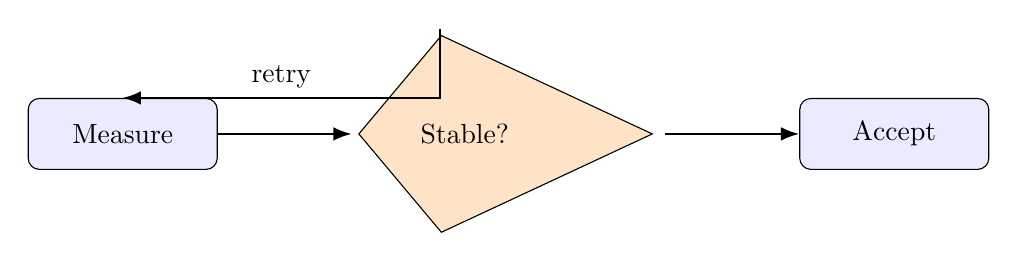
\begin{tikzpicture}[
  >=Latex,
  node distance=17mm,
  process/.style={draw,rounded corners,minimum width=24mm,minimum height=9mm,fill=blue!8},
  gate/.style={kite,shape border rotate=90,kite vertex angles=100 and 50,
    draw,fill=orange!22,minimum width=25mm,minimum height=18mm,outer sep=2pt},
  flow/.style={->,thick}
]
  \node[process] (read) {Measure};
  \node[gate,right=of read] (check) {Stable?};
  \node[process,right=of check] (save) {Accept};

  \draw[flow] (read) -- (check);
  \draw[flow] (check.lower vertex) -- (save);
  \draw[flow] (check.right vertex) |- node[above,pos=.75]{retry} (read.north);
\end{tikzpicture}
\end{document}
